\documentclass[10pt]{article}
\usepackage{amsmath}
\usepackage{amssymb}
\usepackage{setspace}
\usepackage{tasks}
\usepackage{graphicx}
\usepackage{float}
\usepackage{listings}
\usepackage[utf8]{inputenc}
\usepackage{amsfonts}
\usepackage{gensymb}
\usepackage{multicol}
\usepackage{tabularx}
\usepackage{tikz}
\usetikzlibrary{arrows,shapes,automata,petri,positioning,calc}
\usepackage{hyperref}
\usepackage[margin=0.5in]{geometry}

% Power functions
\newcommand{\myvec}[1]{\ensuremath{\begin{pmatrix}#1\end{pmatrix}}}
\let\vec\mathbf

\newcommand{\mydet}[1]{\ensuremath{\begin{vmatrix}#1\end{vmatrix}}}
\providecommand{\brak}[1]{\ensuremath{\left(#1\right)}}
\providecommand{\lbrak}[1]{\ensuremath{\left(#1\right.}}
\providecommand{\rbrak}[1]{\ensuremath{\left.#1\right)}}
\providecommand{\cbrak}[1]{\ensuremath{\left\{#1\right\}}}
\providecommand{\sbrak}[1]{\ensuremath{{}\left[#1\right]}}
\providecommand{\norm}[1]{\left\lVert#1\right\rVert}
\providecommand{\abs}[1]{\left\vert#1\right\vert}

\begin{document}
\title{\textbf{Triangles}}
\maketitle

\section*{9$^{th}$ Maths - Chapter 7}
This is Problem-5 from Exercise 7.1

\begin{enumerate}
\item Line $l$ is the bisector of an angle $\angle{A}$ and $B$ is a point on line $l$. $BP = BQ$ are perpendiculars from $B$ to the arms of $\angle{A}$. 
\begin{enumerate}
\item $\triangle{APB} \cong \triangle{AQB}$
\item $BP = BQ$ or $B$ is equidistant from the arms of $\angle{A}$
\end{enumerate}
\end{enumerate}

\textbf{Construction}\\
The input parameters for the construction are shown in Table 
\begin{figure}[H]
    \begin{center}
     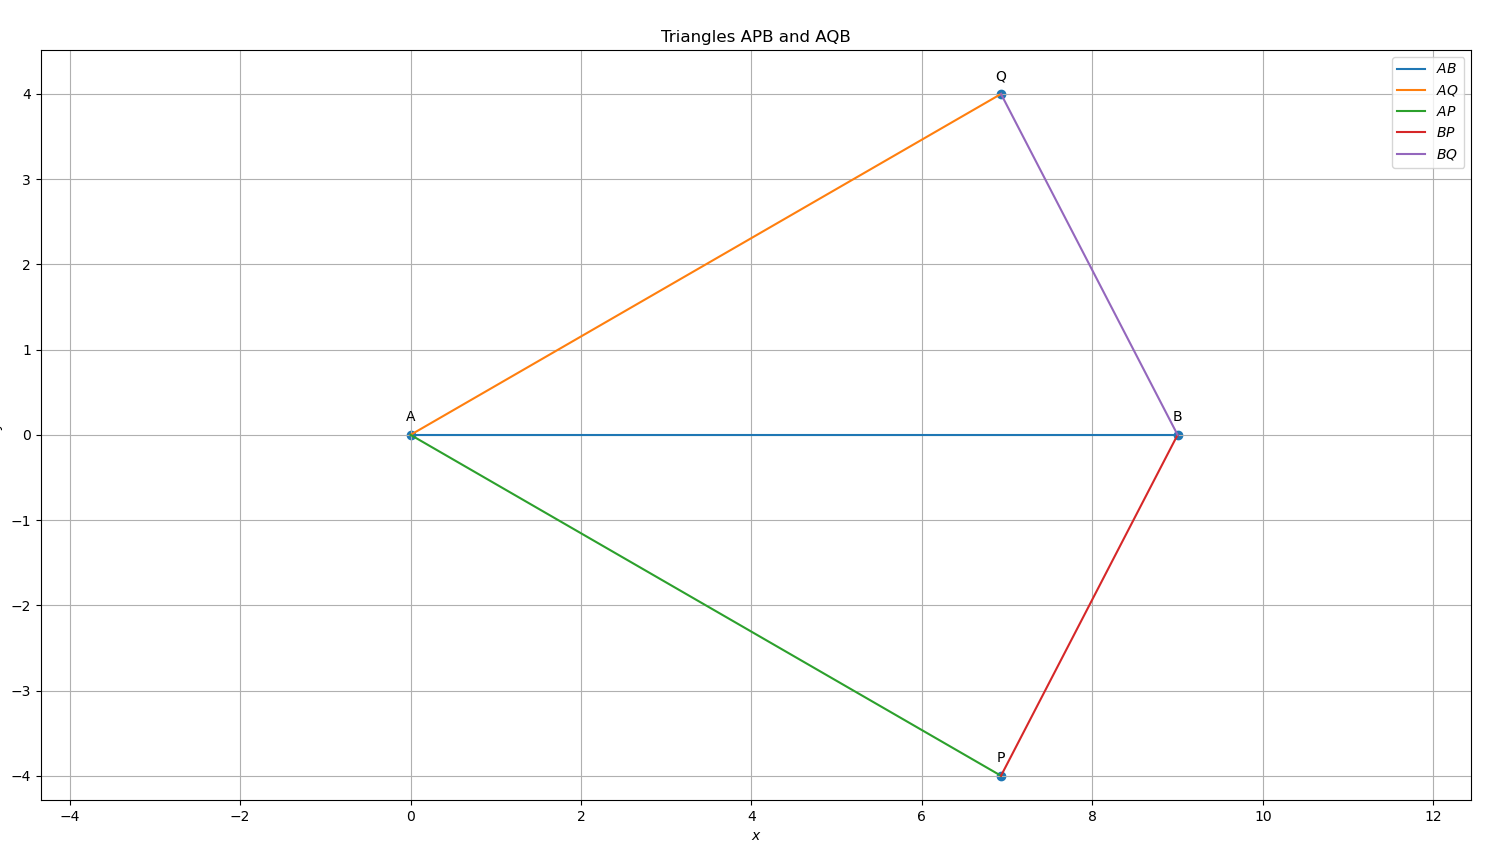
\includegraphics[width=\columnwidth]{figs/tri.png}
    \caption{figure}
    \label{fig1}   
    \end{center}
\end{figure}



\begin{table}[h]
	  \centering
	  \begin{tabular}{|c|c|p{5cm}|}
\hline
\textbf{Symbol} & \textbf{Value} & \textbf{Description} \\
\hline
$\theta$ & $30\degree$ & $\angle{BAP} = \angle{BAQ}$ \\
\hline
$a$ & $9$ & $AB$ \\
\hline
$c$ & $8$ & $AQ$ \\
\hline
$\vec{e}_1$ & $\myvec{1\\0}$ & Basis vector \\
\hline
\end{tabular}

	  \caption{Parameters}
	  \label{Table}
\end{table}

Let $\vec{A} = \myvec{0\\0}$, $\vec{B} = a\vec{e_1}$, $\vec{Q} = \myvec{c\cos\theta\\c\sin\theta}$, and $\vec{P} = \myvec{c\cos\theta\\-c\sin\theta}$.

\section{Solution}
\textbf{Given:}
\begin{align}
\vec{Q}-\vec{A} &= \vec{A}-\vec{P}\\
\angle{QAB} &= \angle{PAB} \\
\angle{AQB} &= \angle{BPA}\\
AB &= AB \quad (\text{common side})
\end{align}

\textbf{To prove:}
\begin{enumerate}
\item $\triangle{APB} \cong \triangle{AQB}$
\item $BP = BQ$ or $B$ is equidistant from the arms of $\angle{A}$
\end{enumerate}

\textbf{Proof:}
\begin{align}
\angle{QAB} &= \angle{PAB}\\
\angle{AQB} &= \angle{BPA}
\end{align}

$AB$ is the common side of $\triangle{APB}$ and $\triangle{AQB}$. Therefore, by A-A-S rule, $\triangle{APB} \cong \triangle{AQB}$. 

\begin{align}
\norm{\vec{B}-\vec{P}} &= \norm{\myvec{9\\0} - \myvec{8\cos\theta\\-8\sin\theta}} = \norm{\myvec{2.07 \\ 4}} = 4.4\\
\norm{\vec{B}-\vec{Q}} &= \norm{\myvec{9\\0} - \myvec{8\cos\theta\\8\sin\theta}} = \norm{\myvec{2.07 \\ -4}} = 4.4\\
\norm{\vec{B}-\vec{P}} &= \norm{\vec{B}-\vec{Q}}
\end{align}

Therefore, $BP = BQ$ or $B$ is equidistant from the arms of $\angle{A}$ is proved.

\end{document}
